\chapter{Ultrafast Ultrasound Imaging}
\label{chap:ultrafast_ultrasound}
% Conventional ultrasound has been used for clinical examination since the 1970s. Conventional ultrasound works 
Although the title of this literature survey and the title of this chapter would suggest that we would dive right in the domain of \textit{ultrafast} ultrasound, I first will briefly introduce the conventional technology. This makes it easier to understand the fundamental differences between the two technologies, that may seem closely related on first sight. 

Conventional ultrasound is based on the principles used in underwater sonar imaging. In conventional ultrasound imaging, a focused beam is generated and used to insonify the medium at specific locations. Next, the backscattered echo from this focus point is recorded, and used to generate a single vertical line of the image. This process, focused insonification and recording of the backscatter, has to be repeated for the number of desired vertical lines in the image, where more lines result in increased horizontal resolution. On the other hand, ultrafast ultrasound imaging is more similar to concepts used in optical holography \cite{tanter_ultrafast_2014}. Instead of using multiple focused insonifications, ultrafast ultrasound uses a single plane wave (i.e. unfocused) to insonify the complete region of interest in an object. From the backscatter of a single insonification, the complete image can be reconstructed.

Since the object only has to be insonified once, the frame rates for wide (multi-line in conventional ultrasound) images are much higher. The increase in frame rate has a cost, the contrast in the images constructed from a single unfocused insonification is lower than the contrast in images acquired with the conventional (focused) method \cite{sandrin_time-resolved_1999}. However, the imaging with very high frame rates makes it possible to image very fast processes, making the technique applicable for blood flow analysis, elastography and even the measurement of brain activity \cite{tanter_ultrafast_2014}. 

In this chapter, the working principle of ultrafast ultrasound will be explained, techniques to enhance the image quality will be shown and the (current) main clinical applications, elastography and Doppler ultrasonography, will be discussed. Furthermore, the limitations of this technology will be shown and compared to the conventional ultrasound imaging technique.




% =======================================================================
\section{Image acquisition}
To acquire an image using ultrasound, first an ultrasound wave is generated by a transducer and emitted into the object to be imaged. This wave will partially be transmitted, reflected, refracted and absorbed by the medium \cite{pillen_ultrasonography_2013}. The portion of the wave that is reflected or scattered by means of refraction will return to the transducer, where the resulting wave, i.e. backscatter, can be measured. The backscattered echoes can be used to construct an image of the medium, based on the time of arrival and amplitude of the ultrasound waves. 

Conventional and ultrafast ultrasound both work according to this principle, however, there is a big difference in the used wave front to insonify the medium and the processing of the backscattered echoes to an interpretable image. To fully show the critical difference between conventional and ultrafast ultrasound, first the conventional technique will be discussed briefly. 



% -----------------------------------------------------------------------
\subsection{Conventional Ultrasound Imaging}
In conventional ultrasound imaging, a focused wave front is transmitted into the medium. This focused wave front is generated by sequentially activating the piezoelectric elements in the ultrasound transducer and by tuning the delays, the focus point can be directed (see \autoref{fig:us_focus_beam}). When this focused beam hits an interface, some of the energy will be reflected, and the reflection will be measured by the piezoelectric elements in the transducer. From this measurement a single vertical `line' of the image can be reconstructed. This procedure is performed multiple times, and the individual line shaped images are combined into the resulting ultrasound image (see \autoref{fig:us_line-by-line}). 


% Figures conventional ultrasound
\begin{figure}[t]
% \centering
\begin{minipage}[t]{.48\textwidth}
  \centering
  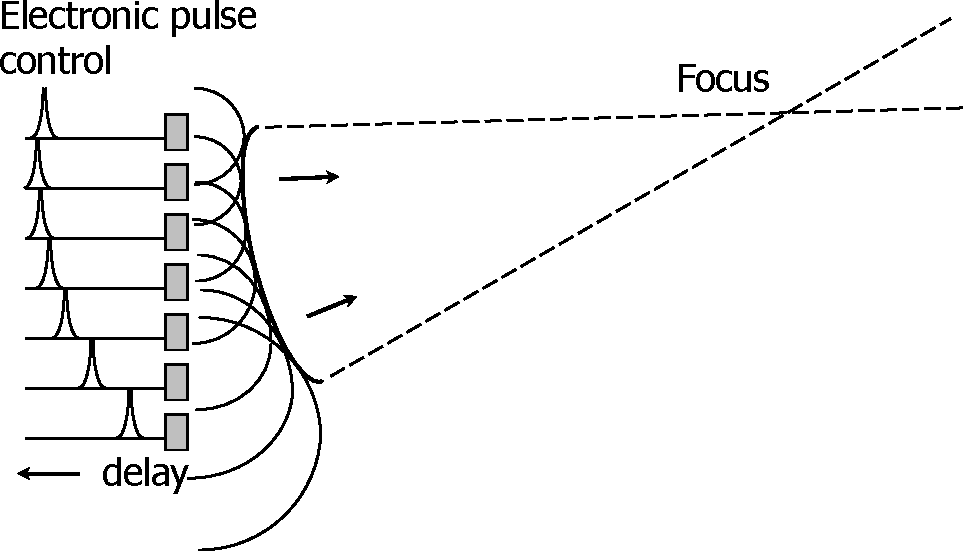
\includegraphics[width=.9\linewidth]{Figures/Ultrasound/ultrasound_focused_beam_v2.pdf}
  \captionof{figure}{Generating a focused wave front by adjusting the delays at which the individual piezoelectric elements in the transducer generate the ultrasound wave. The focus point can be directed at an arbitrary location.}
  \label{fig:us_focus_beam}
\end{minipage} $\quad$
\begin{minipage}[t]{.48\textwidth}
  \centering
    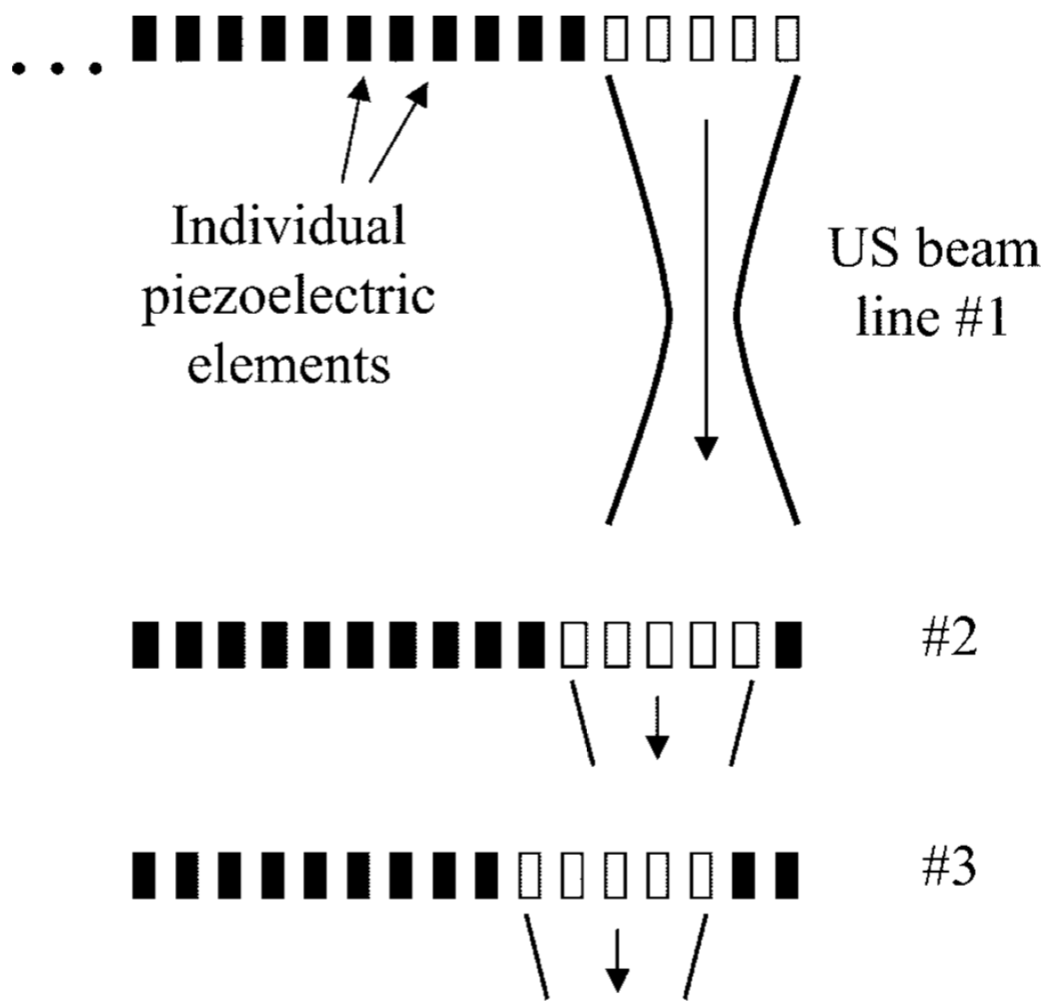
\includegraphics[width=.75\linewidth]{Figures/Ultrasound/conventional_line_scanning.png}
    \caption{The process of line-by-line scanning in conventional ultrasound. The imaging speed depends both on the depth of the object to image (acoustic travel time) and on the number of lines to scan (width of the resulting image). Figure adapted from \citet{hangiandreou_aapm/rsna_2003}.}
    \label{fig:us_line-by-line}
\end{minipage}
\end{figure}


% The process acquiring an image in the conventional method by generating a focused beam, measuring its reflection, and repeating this for the number of desired horizontal image lines, 
The described process of acquiring the ultrasound image, is also known as line-by-line scanning. The frame rate of this conventional method is limited by the number of desired scanning lines and the depth of the object to image. The time it takes to acquire one image is given by,
\begin{equation}
    T_\text{image} = \frac{2 \, z \, N_\text{lines}}{c},
\end{equation}
with $z$ the depth of the object to image, $N_\text{lines}$ the number of lines and $c$ the speed of sound through the medium, usually around \SI{1540}{\meter\per\second} in soft tissue. This already shows that the imaging frame rate for superficial tissue at e.g. \SI{5}{\centi\meter} with 256 lines is limited to \SI{60}{\hertz}. 

There have been several attempts to speed up the imaging speed in conventional ultrasound, for example a technique called ``explososcan''. With this technique, a slightly unfocused beam is emitted, and the recorded echo can be used to parallel process 4 lines from one transmit \cite{shattuck_explososcan_1984}. This increases the imaging speed by a factor four, at cost of image quality. However, for some applications, e.g. tracking and analysis of heart motion, this increase in frame rate is insufficient. 




% -----------------------------------------------------------------------
\subsection{Plane wave ultrafast ultrasound}
Ultrafast ultrasound (or plane wave ultrasound) uses plane waves (i.e. unfocused waves) to insonify the complete region of interest. Part of the plane wave will be reflected or scattered by the object, and the resulting backscattered echoes are recorded by the piezoelectric elements in the transducer. Each element records a different echo and converts the sound waves to Radio Frequency (RF) signals. These RF signals can then be used to reconstruct the image of the insonified object, due to the fact that acoustic waves can be time reversed. Although this may sound very similar to the conventional method, the underlying principle from physics is very different. Since there is no need for a focussed wave, the entire image can be acquired from a single insonification by parallel beamforming of the RF data. This speeds up the image acquisition time tremendously. 
%This appears similar to conventional ultrasound, however, since there is no need for a focused wave, all lines of the image can be acquired at the same time by parallel beamforming, speeding up the image acquisition time tremendously. 
% via a technique called time reversal. 

\subsubsection{Time reversal of acoustic waves}
The time reversal technique is based on the fact that the propagation of ultrasonic and sonic acoustic waves is a reversible process \cite{tanter_time_2009}. This phenomenon is utilised in the Time Reversal Mirror (TRM), which is made of an array of reversible transducers (e.g. a surface covered with piezoelectric elements in case of ultrasound). From any given emitting source, the TRM first records the emerging waves into memory, after which these recordings are time reversed, and the reversed recording is then transmitted by the TRM transducers (i.e. first in, last out). This will result in the exact reverse of the emitted wave field, as depicted in \autoref{fig:us_time_reversal_mirror}, with presence of an arbitrary obstacle. 

\begin{figure}[t]
    \centering
    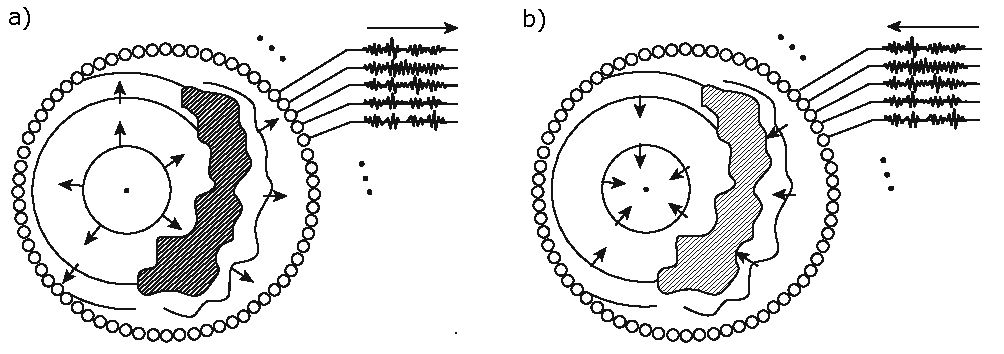
\includegraphics[width=\linewidth]{Figures/Ultrasound/time_reverval_mirror_2.pdf}
    \caption{\textbf{(a) Receiving:} The acoustic waves emitted by a point in the centre travel through the medium, resulting in a distorted wave front, which is then recorded by the Time Reversal Mirror (cylindrical array of piezoelectric transducers). \textbf{(b) Transmitting:} Next the recording is reversed (i.e. time reversal step), and is emitted by the transducers. The wave field will travel through the object, and will refocus exactly at the location of the initial source. Figure adapted from \citet{tanter_time_2009}.}
    \label{fig:us_time_reversal_mirror}
\end{figure}


In the discussed case, a propagating wave field is first recorded and then re-emitted to obtain the reverse field. Due to the reversibility of propagating acoustic waves, the inverse is also possible, i.e. first emitting a wave field and subsequently recording the echoes. Instead of physically generating the time reverse of the wave field, it is also possible to computationally reconstruct what caused the backscattered echo, based on one transmission of a known wave field, by performing digital parallel beamforming of the echoes \cite{tanter_ultrafast_2014}.




\subsubsection{Digital parallel beamforming}

\begin{figure}[!b]
    \centering
    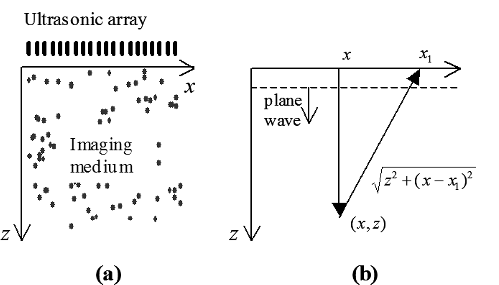
\includegraphics[width=.5\linewidth]{Figures/Ultrasound/beamforming_geo.pdf}
    \caption{Overview of the geometry for calculation of the time delays for a plane wave for an arbitrary point at $(x,y)$ and a transducer located at point $x_1$. Figure adapted from \citet{montaldo_coherent_2009}.}
    \label{fig:us_beamforming_geo}
\end{figure}

% In order to get from raw recorded RF signals to an image, the echoes are numerically backpropagated by a technique called (digital) parallel beamforming (PBF) \cite{tanter_ultrafast_2014}. 
% \textcolor{red}{This method is already fairly old, and newer and better have been developed (e.g. minimum variance beamforming \cite{holfort_plane_2008}). These will not be discussed, because of the complexity of these methods.}
In order to get from raw recorded RF signals to an image, the recorded echoes of the individual elements are beamformed using e.g. the \textit{delay-and-sum} method (DAS, also D\&S or DS). Since there is no focusing in plane wave ultrasound, the image has to be reconstructed by coherently summing the backscattered echoes. For a point $(x,y)$ the travelling time to this point and from this point back to element $i$ at $x_i$ is given by,
\begin{equation}
    \tau \left( x_i, x, z \right) = \frac{z + \sqrt{z^2 + {\left( x- x_i \right)}^2 }}{c},
\end{equation}
with $c$ the speed of sound, assumed constant in the medium \cite{montaldo_coherent_2009}. This situation is depicted in \autoref{fig:us_beamforming_geo}. Each pixel in the image will be reconstructed by first delaying the RF signals with a cylindrical time delay (based on the transducer location with respect to the pixel location), and then coherently summing the delayed signals of each transducer with an aperture weighting \cite{tanter_ultrafast_2002}. For a transducer with $N$ elements, with each element $i$ receiving RF signal $r_i(t)$, the beamformed RF signal from line $x$ becomes, 
\begin{equation}
    r_{BF} \left( x, z\right) = \sum_{i=0}^{N-1} \alpha\left(i,x,z \right) r_i \left(  t \left( x_i, x, z \right) \right),
\end{equation}
with $\alpha(i,x,z)$ the apodization factor, depending on the location of the pixel to beamform and the element number \cite{holfort_broadband_2009}. The apodization factor weights for each pixel to reconstruct how much the raw RF signal from the individual elements has to contribute. In DAS beamforming, the apodization factor is usually based on element directivity. Incident waves with a large angle (large deviation from the perpendicular) are penalised due to their low signal-to-noise ratio (SNR) \cite{chen_improved_2018}. % In general, probe elements are more sensitive to waves with small angular deviation from the perpendicular (,  \cite{chen_improved_2018}.
% which means that elements are more sensitive to waves received at small angles \cite{chen_improved_2018}.

More recently developed beamformers, such as the \textit{minimum variance} (MV) beamformer \cite{holfort_plane_2008}, the \textit{delay multiply and sum} (DMAS) beamformer \cite{matrone_delay_2015} and \textit{Stolt's f-k migration} \cite{garcia_stolts_2013} have proven to be able to reconstruct images with better resolution and contrast than the conventional DAS beamformer. The differences are mostly caused by using data dependent apodization weights, instead of fixed apodization weights based on merely the pixel location and transducer element as used in DAS. The adaptive MV beamformer, uses apodization weights based on the frequency content of the recorded RF signals, and continuously updates these weights \cite{holfort_plane_2008}. The DMAS is a nonlinear beamformer, taking the spatial cross-correlation among all the recorded RF signals of all the transducers at each time instant \cite{matrone_delay_2015}. This again results in a data dependent beamforming by using a measure for the backscattered signal coherence. %\textcolor{red}{\textit{Stolt's f-k migration} \cite{garcia_stolts_2013}}

% \typeout{msg}
% XXX note: use image Montaldo (\cite{montaldo_coherent_2009})?
\bigskip




% -----------------------------------------------------------------------
\subsection{Enhancing image quality}
A disadvantage of plane wave imaging is the loss in contrast and resolution, which is caused by the lack of focus in the transmitted wave \cite{montaldo_coherent_2009}. In order to improve the image quality, various compound imaging methods can be used. 


\subsubsection{Incoherent wave compounding}
By incoherently combining several consecutive frames the effect of noise can be reduced, similar to time domain averaging resulting in increased signal-to-noise ratio. This method is also referred to as real-time spatial compound imaging. Each individual frame is formed of a plane wave under an angle, by means of electronic beam steering. The waves are emitted in a predetermined sequence of angles, usually between 3 an 9 different angles. Next, the frames are combined into an image as depicted in \autoref{fig:us_spatial_compounding}. By having multiple viewing angles, artefacts resulting from one specific view angle are suppressed by the averaging step \cite{entrekin_real-time_2001}. This results in images with less speckle, clutter and other acoustic artefacts. The frame rate is not reduced, since previous recorded frames will be used to enhance the new frame. This can however lead to blurry images, when the tissue or transducer is moving too fast. Since the waves are emitted under an angle, not the entire image can be compounded, meaning that the edges of the image might still contain artefacts \cite{entrekin_real-time_2001}. 

\begin{figure}
    \centering
    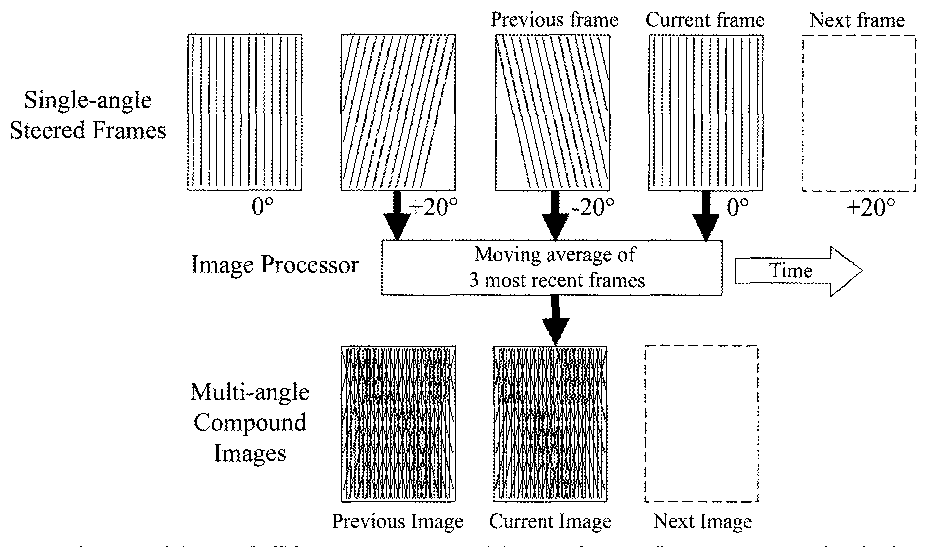
\includegraphics[width=.8\linewidth]{Figures/Ultrasound/spatial_compounding.pdf}
    \caption{Incoherent compound imaging, or real-time spatial compound imaging. Individual frames are made from a single plane wave under an angle. The new image will be composed of the newest acquired frame and the previous $n-1$ frames, with $n$ representing the number of different angles, typically between 3 and 9. Figure adapted from \citet{entrekin_real-time_2001}.}
    \label{fig:us_spatial_compounding}
\end{figure}



\subsubsection{Coherent wave compounding}
In coherent wave compounding, not a combination of beamformed frames is used to create an enhanced image, but the raw received backscattered echoes (RF signals) of multiple plane wave transmits under an angle are combined. The transmit and receive process is similar to incoherent plane wave compounding, but the processing of the received echoes is different. By emitting plane waves under a sequence of angles, the lack of focus can artificially be compensated. By changing the delays of the individual received echoes and summing them coherently, focusing can be performed synthetically at any arbitrary location as depicted in \autoref{fig:us_coherent_compounding}. 

When coherent compounding, the image cannot be formed in real-time, since first all the backscattered echoes need to be recorded, after which the synthetic focusing has to take place. This is a computationally very demanding process and therefore hard to implement in real-time imaging \cite{yiu_gpu-based_2011}. It also reduces the frame rate by the number of angles used. Therefore, for each specific application there is a trade-off in image contrast and resolution versus frame rate. The influence of the number of angles on the image quality is illustrated in \autoref{fig:us_compound_num_angles}. Like in incoherent wave compounding, imaging of fast moving objects can result result in blurry images, though there are methods proposed to compensate for motion using tissue Doppler imaging to estimate the motion of the tissue between successive transmits \cite{poree_high-frame-rate_2016}. 

\begin{figure}
	\centering
	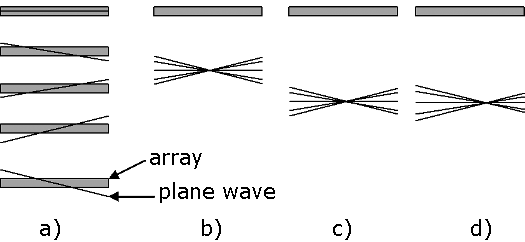
\includegraphics[width=.6\linewidth]{Figures/Ultrasound/coherent_compounding.pdf}
	\caption{In coherent compound imaging focusing can be performed synthetically, by adding the echoes of plane waves with adequate delays. \textbf{(a)} plane waves are emitted under different angles, \textbf{(b)}, \textbf{(c)}, \textbf{(d)} by tweaking the delays the focus point can be changed in both lateral and axial direction. Figure adapted from \citet{montaldo_coherent_2009}.}
	\label{fig:us_coherent_compounding}
\end{figure}


\begin{figure}
    \centering
    \includegraphics[width=\linewidth]{Figures/Ultrasound/compound_num_angles.pdf}
    \caption{Comparison of the effect of coherent plane wave compounding with multiple angles on image quality. The numbers below the number of planes represent the frame rate. Figure adapted from \citet{montaldo_coherent_2009}.}
    \label{fig:us_compound_num_angles}
\end{figure}





% =======================================================================
\subsection{Ultrafast ultrasound compared to conventional ultrasound}
As shown before, ultrafast ultrasound can be a lot faster than conventional ultrasound, due to the fact that the image is acquired by one single plane wave insonification, instead of multiple focused beams. This reduces the acquisition time of the image by the number of scanning lines used in the conventional method. Therefore, the (theoretical) minimum acquisition time per frame in the ultrafast case becomes, 
\begin{equation}
	T_\text{image} = \frac{2 \, z}{c},
\end{equation}
thus only dependent on the imaging depth. In \autoref{tab:us_conv_plane_wave_theoretical_comp}, the theoretical frame rate of conventional and ultrafast ultrasound is stated for a number of clinical applications. Imaging with unfocused waves has a disadvantage. If a plane wave image is compared to a line-by-line scanned image, the plane wave image is of lower quality. To improve the image quality, compound imaging can be used, at cost of frame rate. 


% Table generated by Excel2LaTeX from sheet 'Sheet1'
\begin{table}[t]
  \centering
  \caption{Comparison of theoretical imaging rate for different clinical applications. Conventional ultrasound frame rates are based on 128 scanning lines. Table adapted from \citet{minin_ultrafast_2011}.}
    \begin{tabular}{lccc}
    \toprule
    \multicolumn{1}{p{8.18em}}{Application} & \multicolumn{1}{p{7.5em}}{Typical imaging depth [cm]} & \multicolumn{1}{p{7.5em}}{Conventional frame rate [Hz]} & \multicolumn{1}{p{8.5em}}{Ultrafast imaging rate [Hz]} \\
    \midrule
    Abdominal imaging & 20    & 20    & 3800 \\
    Cardiac imaging & 15    & 150   & 5000 \\
    Breast imaging & 5     & 60    & 15000 \\
    \bottomrule
    \end{tabular}%
  \label{tab:us_conv_plane_wave_theoretical_comp}%
\end{table}%



% Table generated by Excel2LaTeX from sheet 'Sheet1'
\begin{table}[t]
  \centering
  \caption{Comparison of different imaging techniques. Table adapted from \citet{montaldo_coherent_2009}.}
    \begin{tabular}{lcccc}
    \toprule
          & \multicolumn{1}{l}{Resolution [mm]} & \multicolumn{1}{l}{Frame rate [Hz]} & \multicolumn{1}{l}{Contrast [dB]} & \multicolumn{1}{l}{SNR [dB]} \\
    \midrule
    Line scanning (128 lines) & 1.1   & 100   & 32    & 18 \\
    Plane wave & 1.8   & 12500 & 12    & 0 \\
    Compound 12 & 1.1   & 1000  & 20    & 11 \\
    Compound 45 & 1.1   & 270   & 30    & 16 \\
    Compound 71 & 1.1   & 176   & 33    & 18 \\
    \bottomrule
    \end{tabular}%
  \label{tab:us_conv_plane_wave_comparison}%
\end{table}%

In \autoref{tab:us_conv_plane_wave_comparison} plane wave imaging is compared with coherent compound imaging and conventional line-by-line scanning. The methods are compared in resolution and contrast (i.e. image quality), frame rate and SNR (relative to single plane wave imaging). The comparison is based on a superficial tissue mimicking phantom (focus depth approx. \SI{30}{\milli\meter}). From the table it becomes clear that coherent compound imaging using 45 angles gives similar image quality as conventional ultrasound, but with improved frame rate. It should be noted that \citeauthor{montaldo_coherent_2009} used a conventional DAS beamformer \cite{montaldo_coherent_2009}. More recently developed beamformers further improve the image quality, meaning that less angles have to be used to reach similar contrast and resolution \cite{chen_improved_2018}.




% =======================================================================
\section{Applications}
The ultrafast imaging rate of plane wave ultrasound has opened up possibilities in multiple clinical applications; elastography, blood flow analysis and functional brain imaging. In this section, these new possibilities will be introduced. Since it is expected that elastography can be useful in system identification experiments, this application is discussed more in depth. The other applications, blood flow analysis and measuring brain activity, are only discussed briefly. 



% -----------------------------------------------------------------------
\subsection{Ultrafast Doppler Blood Flow Analysis}
In conventional ultrasound, two Doppler modes for blood flow analysis are available. The first mode, spectral analysis Doppler, is based on the spectral analysis of the received Doppler signal with respect to some excitation signal, a pulsed wave (PW) or continuous wave (CW). In this mode, measures such as peak flow velocity as function of time, mean flow velocity as function of time and resistance of the artery can be obtained. These measures require high frequent imaging, and thus a high temporal resolution is required which in conventional ultrasound results in a low spatial resolution. As a consequence of the limited frame rate in conventional ultrasound, in spectral analysis Doppler only one location is scanned (or multiple locations along the same line, i.e. multigating). The second mode is colour-coded flow velocity imaging, in which mean flow velocities over a larger region of interest (ROI) can be measured. Due to the higher required spatial resolution, the temporal resolution is lower. Hence, colour flow imaging results in a more qualitative measurement, mostly used to detect abnormalities in the blood flow pattern \cite{tanter_ultrafast_2014}. % In the second mode, colour flow imaging (CFI), the spatial resolution is higher at cost of temporal resolution. By scanning multiple lines a region of interest (ROI) can be analysed, but only mean flow velocities can be measured. Hence it is more a qualitative measurement, 

Physicians ideally use both these Doppler modes and normal imaging (B-mode) simultaneous in real-time, which is impossible with conventional ultrasound. Fortunately, the high frame rates of plane wave ultrasound open up new possibilities, allowing imaging and quantitative blood flow measurements simultaneously \cite{minin_ultrafast_2011}. By performing the Doppler analysis after the image acquisition, the physician is able to adjust the position of the PW Doppler ROI digitally after the exam, instead of manually moving the transducer or selecting another ROI during the examination. Consequently, multiple ROIs can be selected in the recorded image, without the need for successive exams, resulting in shorter examinations for the patient \cite{tanter_ultrafast_2014}. Furthermore, ultrafast ultrasound improves the sensitivity of the blood flow measurement significantly \cite{minin_ultrafast_2011}. 
% It is also possible to create a complete mapping of the vascular system in e.g. the brain. 



% -----------------------------------------------------------------------
\subsection{Ultrafast Doppler Imaging of Brain Activity}
% Standard imaging techniques today allow deep brain imaging (e.g. EEG, PET and fMRI). For example, fMRI can be used to perform functional imaging deep in the brain, even able to measure increases in blood-oxygen levels ...
Another field in which ultrafast ultrasound shows new possibilities is in neuroscience. Standard imaging techniques today allow deep brain imaging (e.g. EEG, PET and fMRI), but their use is limited. These techniques have limitations in temporal resolution and signal-to-noise ratio at high spatial resolutions. Furthermore, the size of the imaging equipment limits its use in the operating room for monitoring brain activity \cite{tanter_ultrafast_2014}. 

Conventional ultrasound (PW Doppler) is not sensitive enough to measure blood flow in small vessels in the brain, but with the introduction of ultrafast ultrasound the sensitivity is significantly increased. By using ultrafast Doppler, plane wave ultrasound can be used to measure subtle changes in blood flow in the brain, which could provide new information regarding stroke \cite{tanter_ultrafast_2014}. The use of ultrafast ultrasound in brain functional imaging is also referred to as fUltrasound, in analogy with fMRI. The disadvantage of fUltrasound is that its use is limited due to the skull distorting or even blocking the propagation of the ultrasound waves. Therefore, the application is currently limited, but shows great potential for monitoring brain activity in newborns through the fontanel window, and in adults duing neurosurgery \cite{tanter_ultrafast_2014}. 




% -----------------------------------------------------------------------
\subsection{Elastography -- Supersonic shear wave imaging}
\label{sec:us_ssi}
Elastography is the first clinical application of ultrafast ultrasound. Elastography is an imaging method used to map tissue stiffness, and has been under development since the 1990's \cite{gennisson_ultrasound_2013}. It was developed to replace manual palpation by clinicians, and shift from qualitative estimation of the elastic tissue properties to a more quantitative estimation. Elastography can be divided in quasi-static and dynamic methods. 

In the quasi-static method, only a qualitative map can be made of tissue strain. Some constant force is externally applied to compress the tissue, resulting in constant stress in the tissue. Ultrasound images (usually conventional line-by-line scanning) are acquired without force present and next with the compressing force. By tracking the displacement of the tissue, a strain map can be generated. Following Hooke's law, $\sigma = E \epsilon$, it is known that the strain is proportional to the stress (assuming that the tissue behaves linear-elastic). Using this method, the Young's modulus $E$ cannot be found, and only a qualitative strain mapping can be made \cite{gennisson_ultrasound_2013}. 

The dynamic methods can be used in a more quantitative way to determine the elastic properties. There are several dynamic elastography methods, vibro-acoustography, acoustic radiation force imaging (ARFI), 1D transient elastography, 2D transient elastography and supersonic shear wave imaging (SSI). Only the latter uses ultrafast ultrasound imaging, the others rely on conventional ultrasound. All methods based on conventional ultrasound face the same limitations as the other discussed applications, i.e. a strict trade-off in temporal resolution versus spatial resolution. %limited temporal resolution at high spatial resolution and vice versa. 
In dynamic elastography a time varying force perturbation (transient or oscillatory) is induced by the ultrasound transducer, or some other (mechanical) transducer. This perturbation will result in a shear wave in the tissue, typically with a frequency between 10 and 2000 \si{\hertz} \cite{gennisson_ultrasound_2013}. By following this shear wave in the acquired ultrasound images, the propagation velocity of the wave can be found. From this, the elastic properties of the tissue can be determined.

In all dynamic elastography methods, the tissue is assumed to behave as a linear elastic material. In purely elastic media, the phase velocity is independent of shear wave frequency. Consequently, when performing dynamic elastography, only the elastic properties of the medium can be estimated. If the material behaves viscoelastic, shear wave spectroscopy (SWS) can be performed, which will be discussed in \autoref{sec:us_sws}.




\begin{figure}[t]
    \centering
    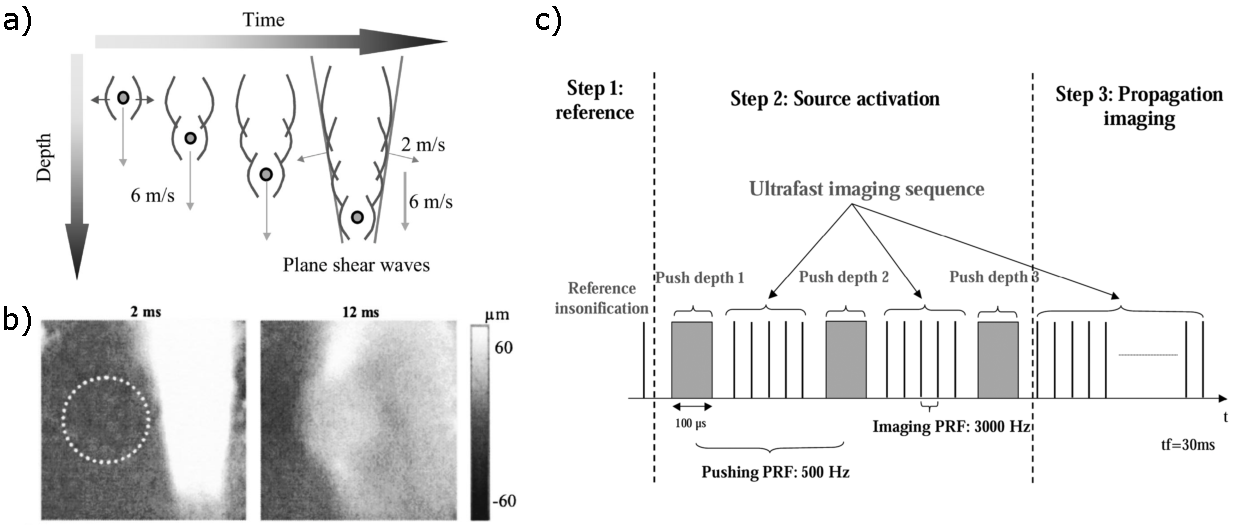
\includegraphics[width=\linewidth]{Figures/Ultrasound/us_shear_wave_imaging.pdf}
    \caption{\textbf{(a)} Generation of the Mach cone by `pushing' multiple focused beams at different depths, constructive interference results in the plane shear wave front. \textbf{(b)} Propagation of the shear wave through a tissue-mimicking phantom (agar-gelatin), with a \SI{20}{\milli\meter} diameter hard inclusion. \textbf{(c)} emission sequence in supersonic shear wave imaging. Figures \textbf{(a,b)} adapted from \citet{bercoff_sonic_2004} and \textbf{(c)} from \citet{bercoff_supersonic_2004}.}
    \label{fig:us_mach_cone}
\end{figure}

% \tred[XXX]
\subsubsection{Supersonic shear wave imaging}
In supersonic shear wave imaging (SSI) the mechanical perturbation that results in the shear wave is induced by the ultrasound transducer using acoustic radiation pressure. The shear wave is created by successively focusing the ultrasonic probe at different depths. Consequently, the resulting shear waves will interfere constructively, and form a Mach cone. In the imaging plane, this can be seen as two shear waves propagating in opposite direction (depicted in \autoref{fig:us_mach_cone}a and b) \cite{bercoff_sonic_2004}. The use of this constructive interference increases the amplitude of the shear wave (compared to single focusing), hence resulting in a higher SNR of the displacement field \cite{gennisson_ultrasound_2013}. The order of displacement is about \SI{40}{\micro\meter} \cite{bercoff_sonic_2004}. Since the induced shear wave travels within the range of 1--10 \si{\meter\per\second}, an imaging rate of minimal \SI{1000}{\hertz} is required to follow this wave \cite{minin_ultrafast_2011}. These frame rates are only possible at high spatial resolution by using ultrafast ultrasound. 
% frequency not too high, otherwise attenuation... ?

The sequence in which SSI is performed is depicted in \autoref{fig:us_mach_cone}c. In the first step, a reference image is formed, used to determine the displacements induced by the shear wave. In the second step, the supersonic source is activated by successive focusing a beam at multiple depths (4 depicted in \autoref{fig:us_mach_cone}a and 3 in \autoref{fig:us_mach_cone}c). After each push at the designated depth, ultrafast imaging can be performed to follow the formation of the Mach cone and propagation of the shear wave. After shear wave pushing is completed, ultrafast imaging can be performed to follow the shear wave. The total sequence for a single SSI measurement takes less than \SI{30}{\milli\second} \cite{bercoff_supersonic_2004}. It should be noted that the first images after generation of the shear wave cannot be used, since the pushing beam itself is backscattered. This blinds the probe momentarily, resulting in approximately   \SI{0.5}{\milli\second} of dead time after shear wave pushing during which no usable images can be reconstructed \cite{deffieux_shear_2009}.
% The difference in propagation speed between compressional waves and shear waves is sufficiently large, that imaging using ultrafast ultrasound does not interfere with the 


\subsubsection{Assumptions from material science}
There are two types of mechanical waves that can propagate through soft tissue: compressional waves (also called longitudinal waves, used for ultrasound imaging) and shear waves. These two types of waves have very different propagation speeds through soft tissue, for compressional waves about \SI{1500}{\meter\per\second} versus about \SI{10}{\meter\per\second} for shear waves. This is caused by the fact that the bulk modulus $\lambda$ of soft tissue is much higher (factor $10^6$) than the shear modulus $\mu$ \cite{minin_ultrafast_2011}. 

Soft tissues are often characterised as fluid-like solids. If it is assumed that soft tissue behaves like an isotropic linear elastic material, its properties can be expressed in terms of two parameters, bulk (compressional) modulus and shear modulus \cite{sarvazyan_biophysical_1995}. Two other mechanical parameters, Young's modulus $E$ and Poisson's ratio $\nu$, are related to $\lambda$ and $\mu$,
\begin{equation}
    \label{eq:K}
    \lambda = \frac{E}{3(1-2\nu)},
\end{equation}
\begin{equation}
    \label{eq:G}
    \mu = \frac{E}{2(1+\nu)}.
\end{equation}
By combining these equations, an expression for the Young's modulus can be found in terms of $\lambda$ and $\mu$, 
\begin{equation}
    E = \frac{9 \mu \lambda}{(\mu + 3 \lambda)}.
\end{equation}
Then using the assumption that the bulk modulus is a factor $10^6$ larger than the shear modulus ($\lambda \gg \mu$), the Young's modulus $E$ (measure for tissue elasticity) can be expressed as,
\begin{equation}
    E = \frac{9 \lambda \mu}{3\lambda + \mu} \approx 3 \mu.
\end{equation}
By using the relation between shear wave propagation speed $c_g$ (group velocity), shear modulus and density of the tissue $\rho$, $\mu = \rho {c_g}^2$, the relation between the Young's modulus and shear wave propagation speed is found,
\begin{equation}
    E = 3 \mu = 3 \rho \, {c_g}^2.
\end{equation}
Concluding, by assuming that soft tissue behaves like an isotropic linear elastic material, the tissues Young's modulus $E$ can be estimated by the propagation speed of a shear wave in tissue. 

In reality, soft tissue is not behaving linear and isotropic, and the elastic moduli are not time invariant. However, according to \citeauthor{sarvazyan_biophysical_1995} this very simplistic model is quite adequate, and depending on the problem can be advantageous over more complex models that require many material parameters \cite{sarvazyan_biophysical_1995}.

% Elastograpgy gaat ervanuit dat alle materialen homogeen / isentroop zijn. tendon (connective tissue) is anisotropic, and anisotropy can cause a different amount of ultrasound reflection, depending on the angle of the incident ultrasound wave. 
% Tegenstrijdig hoe Elastography werkt en imaging van tissue.



\subsection{Elastography -- Shear wave spectroscopy}
\label{sec:us_sws} %\tred 
% \subsubsection{Shear wave spectroscopy}
In linear elastic media, the phase velocity of a shear wave is equal to its group velocity. For viscoelastic media such as breast and liver tissue, the phase velocity increases as a function of frequency (i.e. dispersion), which means that a different rheological model and measurement method has to be used to determine its material properties \cite{minin_ultrafast_2011}. In SSI, the shear modulus $\mu$ can be estimated by merely looking at the wave's group velocity, hence millimeter resolution suffices. SWS on the other hand, relies on estimation of the phase velocity which requires a higher resolution and SNR, since the amount of energy for the individual frequency components is lower than the total energy of the signal \cite{deffieux_shear_2009}. For a high SNR and resolution, it is beneficial to take a relatively large ROI of \SI{1}{\centi\meter\squared}, since smaller ROIs result in a larger variance on the estimation of the shear wave velocity. Within this ROI, the tissue is assumed to be homogeneous for the SWS analysis. Since there is about \SI{0.5}{\milli\second} of dead time after shear wave pushing, it is important to locate the ROI at a lateral distance of approximately \SI{4}{\milli\meter} from the pushing line, allowing imaging of the shear wave propagation in the complete ROI. 

\citeauthor{deffieux_shear_2009} first introduced SWS, by using an experimental setup able to perform one complete SSI experiment within \SI{200}{\milli\second} (\SI{25}{\milli\second} of shear wave pushing and imaging, additional time is required for transferring data, beamforming, speckle tracking and velocity map building) \cite{deffieux_shear_2009}. This setup allowed performing 10 successive SSI experiments in 2 seconds. The 10 acquired velocity fields $u(x,z,t)$ were averaged to increase the SNR. The resulting velocity field was further averaged along the $z$ direction (depth, see \autoref{fig:us_sws_wave_propagation}), to obtain the velocity field $u(x,t)$. Taking the Fourier transform of the velocity field $u(x,t)$ results in $U(x,\omega)$, which can be divided in phase $\varphi(x,\omega)$ and amplitude $A(x,\omega)$ of the wave for each frequency $\omega$ at location $x$. 


% Figures SWS
\begin{figure}[t]
% \centering
\begin{minipage}[t]{.48\textwidth}
  \centering
  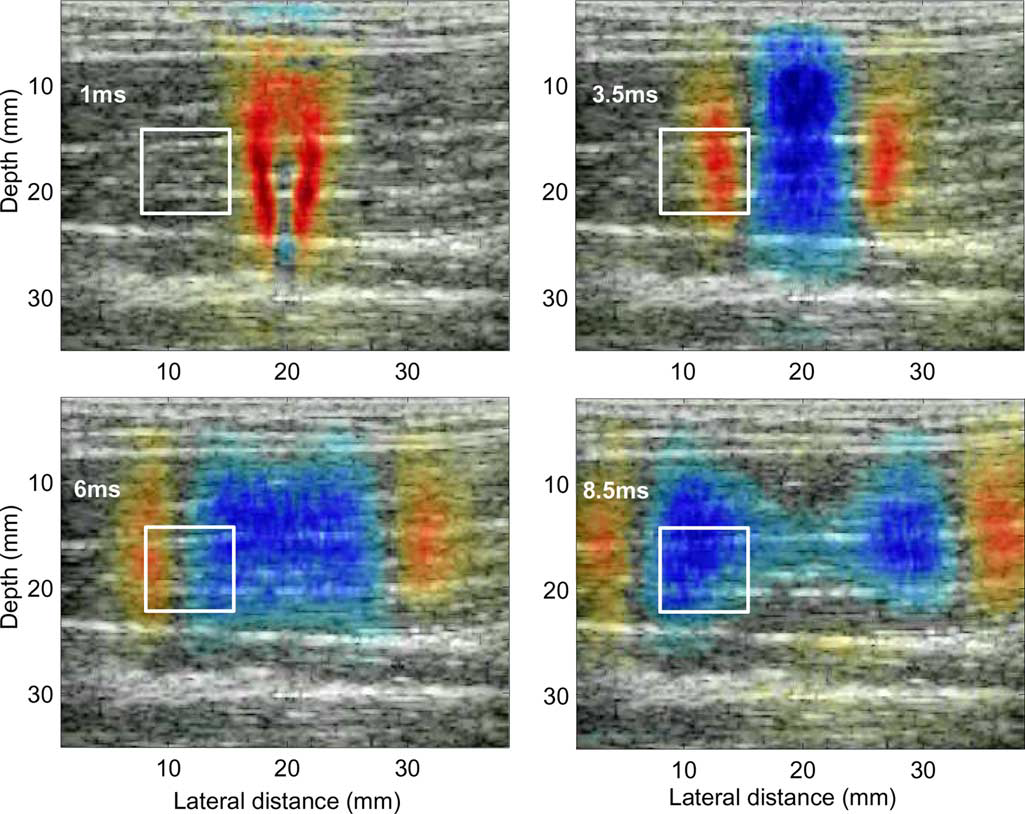
\includegraphics[width=\linewidth]{Figures/Ultrasound/us_sws_wave_propagation_muscle.png}
  \captionof{figure}{Propagation of a shear wave along muscle fibres of the \textit{biceps brachii}. Two quasi-plane waves propagate in opposite direction, causing maximum relative tissue displacement of around \SI{10}{\micro\meter} between successive images at a frame rate of \SI{4000}{\hertz}. The colour scale represents the tissue velocity in the $z$ (depth) direction. The colour scale has been re-normalised for each individual image for clear visualisation of the shear wave, since the amplitude slowly decreases over time. Figure adapted from \citet{deffieux_shear_2009}.}
  \label{fig:us_sws_wave_propagation}
\end{minipage} $\quad$
\begin{minipage}[t]{.48\textwidth}
  \centering
    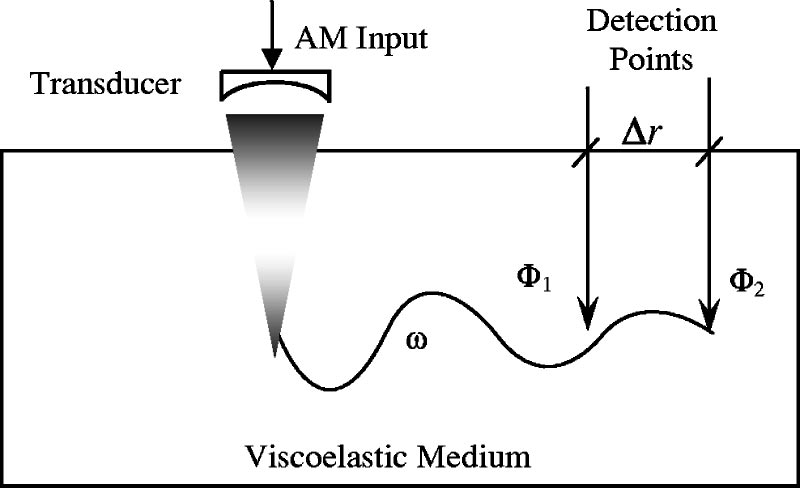
\includegraphics[width=\linewidth]{Figures/Ultrasound/us_sws_phase_diff.png}
    \caption{Concept of shear wave phase velocity estimation. The phase of the wave is measured at two locations at distance $\Delta r$. The shear wave's phase velocity $c_{\varphi}$ can be  determined by the phase shift ($\Delta \varphi = \varphi_1 - \varphi_2$), the frequency of the shear wave $\omega$ and the distance $\Delta r$. Figure adapted from \citet{chen_quantifying_2004}.}
    \label{fig:us_sws_phase_diff}
\end{minipage}
\end{figure}


To determine the phase velocity of the shear wave per frequency, the phase difference of the individual frequency components is determined over a certain distance $\Delta x$ (the width of the ROI). This way the phase velocity for frequency $\omega$ can be approximated by \cite{chen_quantifying_2004},
\begin{equation}
    c_{\varphi}(\omega) = \frac{\omega \, \Delta x}{\Delta \varphi}.
\end{equation}
Using this equation and the obtained phases $\varphi(x,\omega)$, the phase velocity $c_{\varphi}$ can be estimated for all frequency components. From this, the dispersion curves can be formed, and a rheological model can be fitted. The Voigt and Maxwell models are linear descriptions of a viscoelastic medium, comprising of a spring and damper in series (Maxwell) or parallel (Voigt) \cite{chen_quantifying_2004}. The Voigt model is often used to relate the phase velocity and frequency using the density $\rho$, shear elasticity $\mu_1$ and shear viscosity $\mu_2$,
\begin{equation}
    c_{\varphi}(\omega) = \sqrt{\frac{2\left( \mu_1^2+\omega^2 \mu_2^2\right)}{\rho \left( \mu_1 + \sqrt{\mu_1^2 + \omega^2 \mu_2^2} \right)}}.
\end{equation}
Assuming $\rho$ is known (and constant), the mechanical properties of the medium can be estimated by fitting this rheological model to the experimentally obtained dispersion curve \cite{deffieux_shear_2009}. With the estimated viscoelastic parameters, the stress $\sigma$ in the material can then be derived from,
\begin{equation}
	\sigma = \mu_1 \, \epsilon + \mu_2 \, \dot\epsilon,
\end{equation}
with $\epsilon$ the strain in the material. 

To obtain a usable dispersion curve, the generated shear wave should have sufficient bandwidth. The bandwidth of the shear wave is dependent on the properties of the medium, the ultrasound probe design and the insonification parameters (e.g. the angle of the shear wave) \cite{nguyen_assessment_2011}. As a consequence, the bandwidth varies depending on the application, and is reported to be $50-400$~\si{\hertz} in breast applications  \cite{nguyen_assessment_2011} and $100-800$~\si{\hertz} in muscle application (\textit{in vivo biceps brachii}) \cite{gennisson_viscoelastic_2010}.





% Shear wave spectroscopy (SWS) can be seen as an extension of SSI, and can be used to quantify both local shear elasticity and dispersion in real time \cite{deffieux_shear_2009}. 





% , hence a different method has be used to determine the viscoelastic properties. Shear wave spectroscopy
% When the shear wave is properly generated and imaged, the waves phase velocity and group velocity as function of frequency can be determined locally \cite{minin_ultrafast_2011}. For different tissue types, different rheological models can be used. The phase velocity is independent of frequency for purely elastic media, and is equal to the group velocity. On the other hand, and other rheological models can be used, depending on the frequency of the shear wave \cite{minin_ultrafast_2011}.

















% FIGURE TIMING DELAYS PLANE WAVE
% \begin{minipage}[t]{.48\textwidth}
%   \centering
%   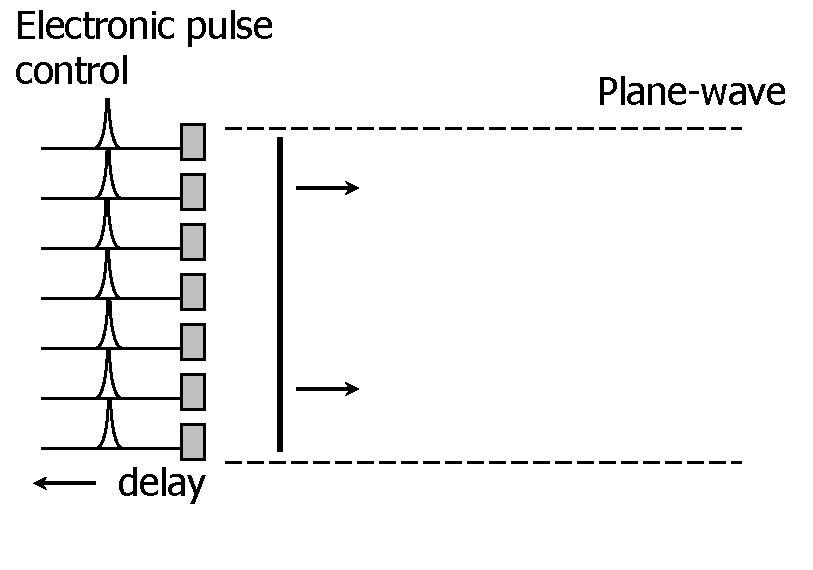
\includegraphics[width=.9\linewidth]{Figures/Ultrasound/ultrasound_plane_wave.pdf}
%   \captionof{figure}{In ultrafast ultrasound imaging a plane-wave front is generated by equal delays on all the piezoelectric elements in the transducer. }
%   \label{fig:us_plane_wave}
% \end{minipage}






% \begin{figure}[H]
%     \centering
%     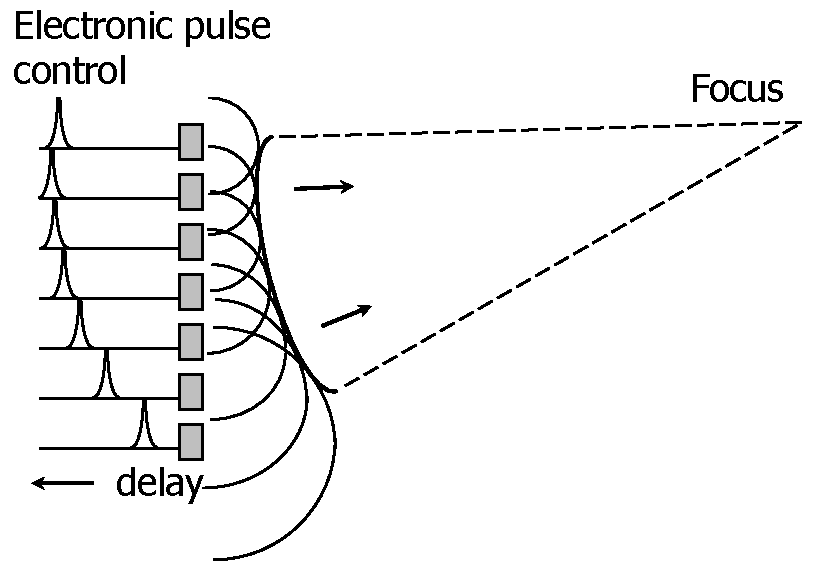
\includegraphics[width=.5\textwidth]{Figures/Ultrasound/ultrasound_focused_beam.pdf}
%     \caption{Generating a focused wave front by adjusting the delays at which the individual piezoelectric elements in the transducer generate the ultrasound wave. The focus point can be directed at any arbitrary location. }
%     \label{fig:us_focus_beam}
% \end{figure}


% \begin{figure}
% \centering
% \begin{subfigure}[t]{.5\textwidth}
%   \centering
%   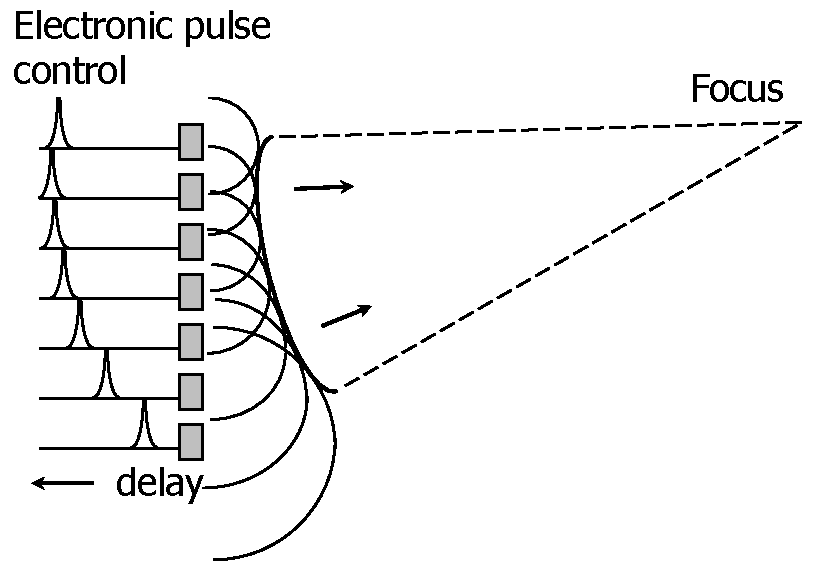
\includegraphics[width=.9\linewidth]{Figures/Ultrasound/ultrasound_focused_beam.pdf}
%   \caption{Generating a focused wave front by adjusting the delays at which the individual piezoelectric elements in the transducer generate the ultrasound wave. The focus point can be directed at any arbitrary location.}
%   \label{fig:us_focus_beam}
% \end{subfigure}
% \begin{subfigure}[t]{.5\textwidth}
%   \centering
%   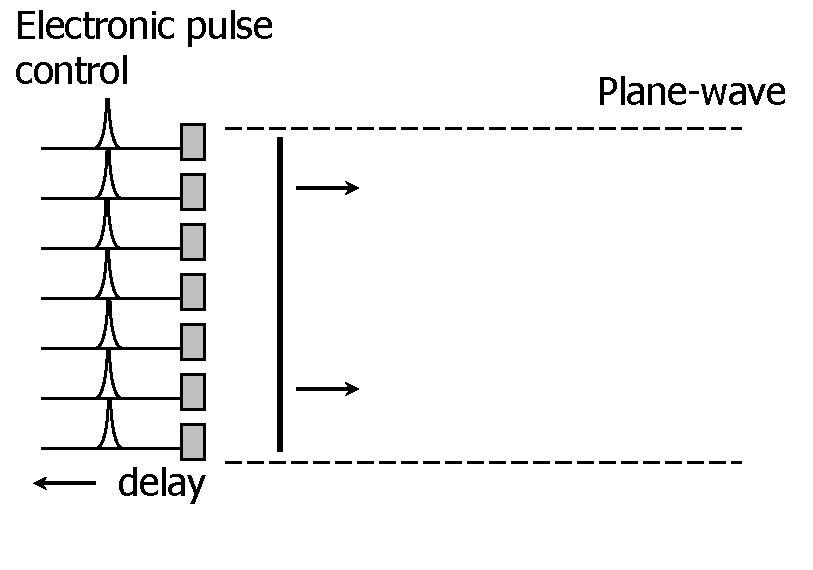
\includegraphics[width=.9\linewidth]{Figures/Ultrasound/ultrasound_plane_wave.pdf}
%   \caption{A subfigure}
%   \label{fig:sub2}
% \end{subfigure}
% \caption{Focused wave-front versus a plane-wave. }
% \label{fig:test}
% \end{figure}